\chapter{Graph Reduction of Lambda\\Expressions}
%\vspace{2cm}
\vspace{1cm}

\noindent
We have now dealt with the issue of which redex to reduce next, and how to
find it. In this chapter we will complete the implementation by showing how to
perform a reduction.

Performing a reduction constitutes a \textit{local transformation} of the graph
representing the expression, so the process of reduction successively modifies
the graph until it reaches its final form, the result of the computation.

As we have seen in the previous chapter, the function at the tip of the spine
may be either a lambda abstraction, or a built-in function (if, that is, the graph
has a top-level redex at all). We will deal with these two cases separately.

\section{Reducing a Lambda Application}

Suppose the redex consists of a lambda abstraction applied to an argument.
Then we must apply the \tb-reduction rule to the graph. That is, we must
construct an instance of the body of the lambda abstraction, substituting the
argument for free occurrences of the formal parameter.

We will sometimes refer to this process as `constructing a new instance of
the body of the lambda abstraction’, but we will often abbreviate this to
`instantiating the lambda body’. Figure~12.1 gives an example.

\boxedfigure{
    \centering
    \raisebox{-\height}{%
        \begin{forest}
            [\ml{@}
                [\ml{\tl x}
                    [\ml{@}
                        [\ml{NOT}]
                        [\ml{x}]
                    ]
                ]
                [\ml{TRUE}]
            ]
        \end{forest}%
    }%
    \raisebox{-\height}{\hspace{1cm}reduces to\hspace{1cm}}%
    \raisebox{-\height}{%
        \begin{forest}
            [\ml{@}
                [\ml{NOT}]
                [\ml{TRUE}]
            ]
        \end{forest}%
    }\\
    \vspace{-\baselineskip}
    \hspace{3cm}
    \ml{(\tlb{x}NOT x) TRUE $\rightarrow$ NOT TRUE}
}{Instantiating the body of a lambda abstraction}

Three important issues of implementation arise here:
\begin{numbered}
    \item The argument may be bulky and/or contain redexes, so we should
    substitute \textit{pointers} to the argument for the formal parameter (see Section~12.1.1).

    \item The redex may be shared, so we must \textit{physically overwrite} the root of the
    redex with the result (see Section~12.1.2).

    \item The lambda abstraction may be shared, so we must construct a \textit{new
        instance} of the lambda body, rather than substituting in the original body
    directly (see Section~12.1.3).
\end{numbered}
We will deal with these issues in the following sections.

\subsection{Substituting Pointers to the Argument}

When substituting the argument for the formal parameter, we could just \textit{copy}
the argument whenever the formal parameter occurred. But copying the
argument may be very wasteful, because
\begin{numbered}
    \item the argument might be a very large expression, in which case we are
    wasting space by making multiple copies of the same object;

    \item the argument might contain redexes, in which case we are wasting work by
    duplicating redexes which may subsequently have to be separately
    reduced (if they are needed).
\end{numbered}
Both of these problems can be avoided by substituting \textit{pointers} to the
argument for the formal parameter. This gives rise to \textit{sharing}, whereby there
may be many pointers to the same expression, and it is for precisely this
reason that the expression tree becomes a graph. Figure~12.2 is an example of
this process in action, in which the \ml{(NOT TRUE)} expression becomes shared.

Sharing by means of pointers was first suggested by Wadsworth~[1971], who
called it \textit{graph reduction}. It is the key idea that turns reduction into a practical
technique. The alternative, of copying the argument wherever it is used, is
called \textit{tree reduction} or \textit{string reduction} and is normally considered
prohibitively expensive (though Mago's parallel reduction machine uses it
[Mago, 1980], relying on massive parallelism to overcome the inefficiency).

\boxedfigure{
    \centering
    \raisebox{-\height}{%
        \begin{forest}
            [\ml{@}
                [\ml{\tl x}
                    [\ml{@}
                        [\ml{@}
                            [\ml{AND}]
                            [\ml{x}]
                        ]
                        [\ml{x}]
                    ]
                ]
                [\ml{@}
                    [\ml{NOT}]
                    [\ml{TRUE}]
                ]
            ]
        \end{forest}%
    }%
    \raisebox{-\height}{\hspace{.5cm}reduces to\hspace{.5cm}}%
    \raisebox{-\height}{%
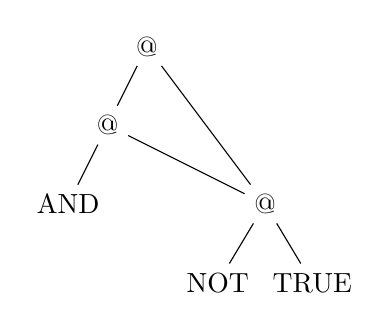
\begin{tikzpicture}
    \node (root) at (0,0) {\ml{@}};
    \node (app1) at (-.5,-1) {\ml{@}};
    \node (app2) at (1.5,-2) {\ml{@}};
    \node (and) at (-1,-2.) {\ml{AND}};
    \node (not) at (.9,-3.) {\ml{NOT}};
    \node (true) at (2.1,-3.) {\ml{TRUE}};

    \draw (root) -- (app1);
    \draw (root) -- (app2);
    \draw (app1) -- (and);
    \draw (app1) -- (app2);
    \draw (app2) -- (not);
    \draw (app2) -- (true);
\end{tikzpicture}
    }\\
    \vs

    \ml{(\tlb{x}AND x x) (NOT TRUE) $\rightarrow$ AND (NOT TRUE) (NOT TRUE)}
}{Pointer substitution}


\subsection{Overwriting the Root of the Redex}

If we are to exploit sharing successfully we must ensure that when an
expression is reduced we modify the graph to reflect the result. This will
ensure that shared expressions will only be reduced once. For instance, in
Figure~12.2 the \ml{(NOT TRUE)} expression will be reduced next (since \ml{AND}
requires its arguments to be evaluated), and we would like to arrange that this
reduction is only done once.

We can achieve this by the simple expedient of physically \textit{overwriting} the
root of the redex with the (root of) the result. Here is an example in which the
node marked `\ml{\$}' is the root of the redex, and is physically overwritten with the
result of the reduction:

\plainbox{
    \centering
    \raisebox{-\height}{%
       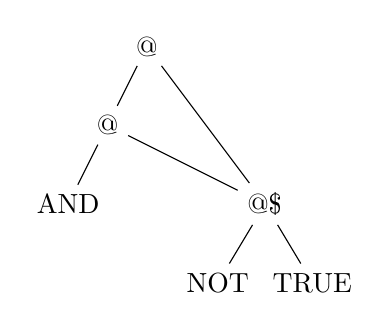
\begin{tikzpicture}
           \node (root) at (0,0) {\ml{@}};
           \node (app1) at (-.5,-1) {\ml{@}};
           \node (app2) at (1.5,-2) {\ml{@\$}};
           \node (and) at (-1,-2.) {\ml{AND}};
           \node (not) at (.9,-3.) {\ml{NOT}};
           \node (true) at (2.1,-3.) {\ml{TRUE}};

           \draw (root) -- (app1);
           \draw (root) -- (app2);
           \draw (app1) -- (and);
           \draw (app1) -- (app2);
           \draw (app2) -- (not);
           \draw (app2) -- (true);
       \end{tikzpicture}%
    }%
    \raisebox{-\height}{reduces to\hspace{0.5cm}}%
    \raisebox{-\height}{%
       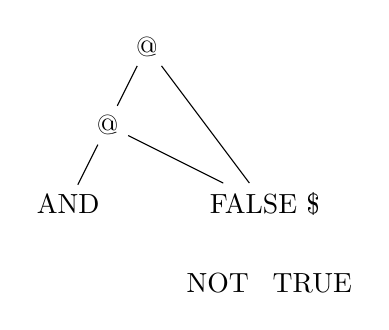
\begin{tikzpicture}
           \node (root) at (0,0) {\ml{@}};
           \node (app1) at (-.5,-1) {\ml{@}};
           \node (app2) at (1.5,-2) {\ml{FALSE \$}};
           \node (and) at (-1,-2.) {\ml{AND}};
           \node (not) at (.9,-3.) {\ml{NOT}};
           \node (true) at (2.1,-3.) {\ml{TRUE}};

           \draw (root) -- (app1);
           \draw (root) -- (app2);
           \draw (app1) -- (and);
           \draw (app1) -- (app2);
%           \draw (app2) -- (not);
%           \draw (app2) -- (true);
       \end{tikzpicture}%
    }
}

Notice that fragments of the redex (in this case just the \ml{NOT} and \ml{TRUE} nodes)
are not affected by the overwriting, and become completely detached from
the part of the graph we are considering. They cannot be recovered and
re-used immediately because they may be shared with other nodes not in the
picture. If not, then they will eventually be recovered by the garbage
collector.

There is an important complication associated with overwriting the root of
the redex, which we discuss later, in Section~12.4.

\subsection{Constructing a New Instance of the Lambda Body}

As the word `instance' implies, when applying a lambda abstraction we must
make substitutions within a \textit{new copy} of the body of the lambda abstraction
rather than updating the original body directly with the substitutions. This is
necessary because the abstraction may be applied many times, and its body
serves as a `master template' from which an instance is constructed each time
it is applied; the master template should not be altered by the copying process.
Thus the example in Figure~12.1 should really look like this:

\plainbox{
    \centering
    \raisebox{-\height}{%
        \begin{forest}
            [\ml{@\$}
            [\ml{\tl x}
            [\ml{@}
            [\ml{NOT}]
            [\ml{x}]
            ]
            ]
            [\ml{TRUE}]
            ]
        \end{forest}%
    }%
    \raisebox{-\height}{\hspace{1cm}reduces to}%
    \raisebox{-\height}{%
        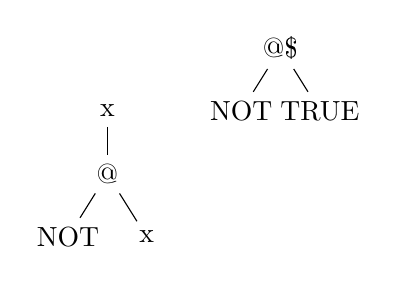
\begin{tikzpicture}[baseline=(tl.base)]
            % Left disconnected tree: lambda abstraction (intact)
            \node (tl)   at (0,0)    {\ml{\tl x}};
            \node (at1)  at (0,-0.8) {\ml{@}};
            \node (not1) at (-0.5,-1.6) {\ml{NOT}};
            \node (x1)   at (0.5,-1.6)  {\ml{x}};
            \draw (tl) -- (at1);
            \draw (at1) -- (not1);
            \draw (at1) -- (x1);
            % Right disconnected tree: new instance (@$)
            \node (ats)  at (2.2, 0.8)  {\ml{@\$}};
            \node (not2) at (1.7, 0)    {\ml{NOT}};
            \node (true) at (2.7, 0)    {\ml{TRUE}};
            \draw (ats) -- (not2);
            \draw (ats) -- (true);
        \end{tikzpicture}%
    }
}

\noindent The original lambda abstraction remains intact in case it is shared.


We may describe the instantiation operation by a recursive function
\ml{Instantiate(Body,Var,Value)}, which copies \ml{Body} substituting \ml{Value} for free
occurrences of \ml{Var}. This function implements precisely the substitution
operation described in Figure~2.3. Specifically:

\begin{mlcoded}
    Instantiate(Body,Var,Value) \quad {\normalfont{\normalsize constructs} }\quad Body[Value/Var]
\end{mlcoded}

\noindent \ml{Instantiate} proceeds by case-analysis on the root node of \ml{Body}, and each case is
a direct transcription of the corresponding line of Figure~2.3:

\begin{numbered}
    \item \textit{if} \ml{Body} is a variable \ml{x} and \ml{Var} $=$ \ml{x} \textit{then} return \ml{Value} (here we substitute
    \ml{Value} for an occurrence of \ml{Var}),
    \item \textit{if} \ml{Body} is a variable \ml{x} and \ml{Var} $\neq$ \ml{x} \textit{then} return \ml{Body},
    \item \textit{if} \ml{Body} is a constant or built-in function \textit{then} return \ml{Body},
    \item \textit{if} \ml{Body} is an application \ml{(E$_1$ E$_2$)} \textit{then} return the application
    \ml{(Instantiate(E$_1$,Var,Value) Instantiate(E$_2$,Var,Value))},
    \item \textit{if} \ml{Body} is a lambda abstraction \ml{\tlb{x}E} and \ml{Var} $=$ \ml{x} \textit{then} return \ml{Body} -- the
    new lambda abstraction binds \ml{Var} anew, so no substitutions should occur
    inside it, and hence we can avoid instantiating it altogether,
    \item \textit{if} \ml{Body} is a lambda abstraction \ml{\tlb{x}E} and \ml{Var} $\neq$ \ml{x} \textit{then} return
    \ml{\tlb{x} Instantiate(E,Var,Value)} -- we must instantiate the lambda abstraction
    in case there are free occurrences of \ml{Var} inside it.\\
    This case is much simpler than the corresponding rule of Figure~2.3,
    because we are assuming that \ml{Value} has no free variables (see Section
    11.3.2).
\end{numbered}

Figure~12.3 gives a possible definition of \ml{Instantiate} in the C language.

The instantiation process is simple enough, but it risks copying large
expressions in which \ml{Var} does not occur free at all, and hence which could be
shared. We could alleviate this by adding a new first clause to the definition of
\ml{Instantiate}:

\vs
\indent \textit{if} \ml{Body} does not contain any free occurrences of \ml{Var} \textit{then} return \ml{Body}.
\vs

\noindent This would, however, be an expensive test to make. We might imagine some
sort of annotation scheme whereby we could precompute such information,
but it is hard to do in general (even Wadsworth did not give an algorithm!).
An implementation which manages to perform this test, or which does
something equivalent, is said to be \textit{fully lazy}. We discuss full laziness in detail
in Chapter~15, but ignore it until then.

\subsection{Summary}

In the previous chapter we saw that lazy evaluation had two ingredients:

\begin{numbered}
    \item arguments to functions should be evaluated only if needed;
    \item once evaluated, they should never be re-evaluated.
\end{numbered}


\boxedfigure{%
    \begin{mlcoded}
        \begin{tabular}{@{}l@{}}
            Instantiate( Body, Var, Value ) \\
            expression *Body, *Var, *Value; \\
            \{ \\
            \quad if (IsAp( Body ))\ \ /* Is Body an application node? */ \\
            \qquad return( MakeAp( Instantiate( GetFun( Body ), Var, Value ), \\
            \qquad \phantom{return( MakeAp( }Instantiate( GetArg( Body ), Var, Value ) ) ); \\
            \\
            \quad if (IsVar( Body )) /* Is Body a variable? */ \\
            \quad \{ \\
            \qquad if (Body == Var) \quad /* Is Body the variable Var? */ \\
            \qquad \quad return( Value ); \\
            \qquad else \\
            \qquad \quad return( Body ); \\
            \quad \} \\
            \quad if (IsLam( Body )) /* Is Body a lambda abstraction? */ \\
            \quad \{ \\
            \qquad if (GetVar( Body ) == Var) \quad /* Same formal parameter? */ \\
            \qquad \quad return( Body ); \\
            \qquad else \\
            \qquad \quad return( MakeLam( GetVar( Body ), \\
            \qquad \phantom{return( MakeLam( }Instantiate( GetBody( Body ), Var, Value ))); \\
            \quad \} \\
            /* So Body must be a constant or built-in function */ \\
            \quad return( Body ); \\
            \} \\[6pt]
            \begin{tabular}{@{}l@{\quad}l@{}}
                Note: & \ml{IsAp(B)} tests whether \ml{B} is an application node \\
                & \ml{GetFun(B)} gets the function from an application node \\
                & \ml{GetArg(B)} gets the argument from an application node \\
                & \ml{MakeAp(F,A)} makes a new application node \\[4pt]
                & \ml{IsVar(B)} tests whether \ml{B} is a variable node \\[4pt]
                & \ml{IsLam(B)} tests whether \ml{B} is a lambda abstraction node \\
                & \ml{GetVar(B)} gets the formal parameter from an abstraction \\
                & \ml{GetBody(B)} gets the body from an abstraction node \\
                & \ml{MakeLam(V,B)} makes a new lambda abstraction node \\
            \end{tabular}
        \end{tabular}
    \end{mlcoded}
}{The \ml{Instantiate} function in C}

\noindent We saw that normal order evaluation implemented the first ingredient. We
can now see that the second ingredient is implemented by the combination of
two things:

\begin{numbered}
    \item substituting pointers to the argument rather than copying it avoids
    duplicating the (unevaluated) argument;
    \item updating the root of the redex with the result ensures that further uses of
    the argument will get the benefit of the work done.
\end{numbered}

\noindent To summarize:

\plainbox{
    \vspace{-\baselineskip}
    \[
    \left.
    \begin{array}{l}
        \text{Normal order evaluation} \\
        \text{to weak head normal form} \\
        \qquad\qquad + \\
        \text{Substitute pointers} \\
        \qquad\qquad + \\
        \text{Update redex root} \\
        \text{with result}
    \end{array}
    \right\}
    = \text{Lazy evaluation}
    \]
}

\noindent This implementation strategy is called \textit{lazy graph reduction}.

\section{Reducing a Built-in Function Application}

Suppose the redex consists of a built-in function applied to the correct number
of arguments. First of all, any arguments whose values are needed must be
evaluated by recursively invoking the evaluator. Then the built-in function
can be executed, and the result physically overwrites the root of the redex.

For example, consider the expression \ml{(+ 6 ($\ast$ 3 4))}, which has the graph

% Shared node positions for both graphs on this page:
% ats  = @$  (0, 0)       -- root
% atl  = @   (-1, -1)     -- left child of root
% atr  = @#  (1, -1)      -- right child of root
% pl   = +   (-1.8, -2)   -- left child of @
% six  = 6   (-0.2, -2)   -- right child of @
% atm  = @   (0.8, -2)    -- left child of @#
% four = 4   (1.8, -2)    -- right child of @#
% str  = *   (0.8, -3)    -- left child of inner @
% thr  = 3   (1.3, -3)    -- right child of inner @

\plainbox{\centering
    \vspace{-0.5\baselineskip}
    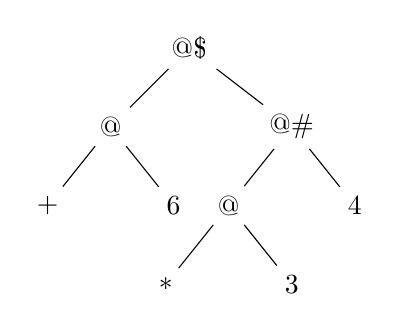
\begin{tikzpicture}
        \node (ats)  at (0,    0)  {\ml{@\$}};
        \node (atl)  at (-1,  -1)  {\ml{@}};
        \node (atr)  at (1.3, -1)  {\ml{@\#}};
        \node (pl)   at (-1.8,-2)  {\ml{+}};
        \node (six)  at (-0.2,-2)  {\ml{6}};
        \node (atm)  at (0.5, -2)  {\ml{@}};
        \node (four) at (2.1, -2)  {\ml{4}};
        \node (str)  at (-0.3, -3)  {$\ast$};
        \node (thr)  at (1.3, -3)  {\ml{3}};
        \draw (ats) -- (atl);
        \draw (ats) -- (atr);
        \draw (atl) -- (pl);
        \draw (atl) -- (six);
        \draw (atr) -- (atm);
        \draw (atr) -- (four);
        \draw (atm) -- (str);
        \draw (atm) -- (thr);
    \end{tikzpicture}
    \vspace{-0.5\baselineskip}
}

\noindent We first select node \ml{\$} for reduction, but discover that \ml{+} needs to evaluate its
arguments. So we recursively invoke the evaluator on the first argument, only
to discover that it is already in WHNF. Then we invoke the evaluator on the
second argument, which causes node \ml{\#} to be selected for reduction. Again,
we recursively reduce the arguments of the $*$ (they are already in WHNF),
and now we can execute the $*$. The result of this multiplication overwrites
node \ml{\#}, thus

\plainbox{\centering
    \vspace{-0.5\baselineskip}
    \begin{tikzpicture}
        \node (ats)    at (0,    0)  {\ml{@\$}};
        \node (atl)    at (-1,  -1)  {\ml{@}};
        \node (twelve) at (1.3, -1)  {\ml{12 \#}};
        \node (pl)     at (-1.8,-2)  {\ml{+}};
        \node (six)    at (-0.2,-2)  {\ml{6}};
        \node (atm)    at (0.5, -2)  {\ml{@}};
        \node (four)   at (2.1, -2)  {\ml{4}};
        \node (str)  at (-0.3, -3)  {$\ast$};
        \node (thr)  at (1.3, -3)  {\ml{3}};
        \draw (ats) -- (atl);
        \draw (ats) -- (twelve);
        \draw (atl) -- (pl);
        \draw (atl) -- (six);
        \draw (atm) -- (str);
        \draw (atm) -- (thr);
    \end{tikzpicture}
    \vspace{-0.5\baselineskip}
}

\noindent As always, we see that fragments of the original graph remain, subsequently
to be recovered by the garbage collector. Now the evaluation of the
arguments of \ml{+} is complete, and it executes, giving

\plainbox{\centering
    \vspace{-0.5\baselineskip}
    \begin{tikzpicture}
        \node (ats)    at (0,    0)  {\ml{18 \$}};
        \node (atl)    at (-1,  -1)  {\ml{@}};
        \node (twelve) at (1.3, -1)  {\ml{12 \#}};
        \node (pl)     at (-1.8,-2)  {\ml{+}};
        \node (six)    at (-0.2,-2)  {\ml{6}};
        \node (atm)    at (0.5, -2)  {\ml{@}};
        \node (four)   at (2.1, -2)  {\ml{4}};
        \node (str)    at (-0.3,-3)  {$\ast$};
        \node (thr)    at (1.3, -3)  {\ml{3}};
%        \draw (ats) -- (atl);
%        \draw (ats) -- (twelve);
        \draw (atl) -- (pl);
        \draw (atl) -- (six);
        \draw (atm) -- (str);
        \draw (atm) -- (thr);
    \end{tikzpicture}
    \vspace{-0.5\baselineskip}
}

\noindent The node \ml{\$}, the root of the original expression, is the result, the other
fragments being garbage. From now on we will no longer draw the garbage
nodes in our pictures.

\section{The Reduction Algorithm So Far}

We now review our reduction algorithm, putting together the material of the
previous two sections.

\plainbox{
    \noindent\ml{REPEAT}
\begin{quote}
    \vspace{-0.5\baselineskip}
    \begin{compactenum}[(1)]
        \item Unwind the spine until something other than an application
        node is encountered.
        \item Examine the objects found at the tip of the spine (see
        Section~11.5).
        \begin{compactenum}[(a)]
            \item \textit{A data object.} Check that it is not applied to anything. If
            not, the expression is in WHNF so \ml{STOP}, otherwise
            there is an \ml{ERROR}.
            \item \textit{A built-in function.} Check the number of arguments
            available. If there are too few arguments the expression
            is in WHNF so \ml{STOP}. Otherwise evaluate any
            arguments required, execute the built-in function and
            overwrite the root of the redex with the result.
            \item \textit{A lambda abstraction.} Check that there is an argument;
            if not the expression is in WHNF so \ml{STOP}. Otherwise
            instantiate the body of the lambda abstraction,
            substituting pointers to the argument for the formal
            parameter, and overwrite the root of the redex with the
            result.
        \end{compactenum}
    \end{compactenum}
    \vspace{-0.5\baselineskip}
\end{quote}
    \ml{END}
}

\section{Indirection Nodes}

In Section~12.1 we described how to reduce an application of a lambda
abstraction by constructing an instance of the body of the lambda abstraction,
substituting pointers to the argument for the formal parameter, and updating
the root of the redex with the result. The final operation, updating the root of
the redex, contains a hidden danger, which this section will expose.

Suppose, then, that we have instantiated the body of the abstraction and
are about to update the root of the redex. The most obvious way to do this
seems to be simply \textit{to copy} the root cell of the result on top of the root cell of
the redex. This is all very well, but it suffers from two shortcomings:

\begin{numbered}
    \item The result of the reduction may not have a root cell to copy. For example,
    consider
    \begin{mlcoded}
    \ml{(\tlb{x}4) 5}
    \end{mlcoded}
    In an unboxed implementation the result, \ml{4}, is represented as a non-
    pointer, and hence does not occupy a cell at all.

    \item It is slightly inefficient, because the root cell of the result is constructed
    (by \ml{Instantiate}), copied over the root of the redex, and then \textit{discarded},
    because there are no further pointers to it.

    \phantom{xx}It would be more efficient to build the root cell of the result directly \textit{on
        top} of the root cell of the redex, thus avoiding ever constructing the root
    cell of the result in the first place.

    \phantom{xx}However, in a reduction such as
    \begin{mlcoded}
        \ml{(\tlb{x}x) (f 6)}
    \end{mlcoded}
    the root cell of the result is \textit{not a newly constructed cell} so we cannot
    construct the root cell of the result on top of the root of the redex.
\end{numbered}

\noindent It appears, therefore, that lambda abstractions in which the body consists of
an unboxed constant or a single variable, form a special case. We consider the
former possibility first.

\subsection{Updating with Unboxed Objects}

We recall from Chapter~10 that an unboxed object is one which is represented
as a non-pointer, rather than as a pointer to a cell. How can we update the root
of the redex with such an object?

We are forced to introduce a new type of cell, an \textit{indirection cell}. An
indirection cell has a tag, \ml{IND} say, which identifies the cell as an indirection,
and a single field which is the contents of the cell. When updating an
application cell with an unboxed object we overwrite the application with an
indirection cell whose content is the unboxed object. For example:

\plainbox{
    \vspace{-0.5\baselineskip}
    \centering
    \raisebox{-\height}{%
        \begin{forest}
            [\ml{@\$}
                [\ml{\tl x}
                    [\ml{4}]
                ]
                [\ml{6}]
            ]
        \end{forest}%
    }%
    \raisebox{-\height}{\hspace{1.5cm}reduces to\hspace{1.5cm}}%
    \raisebox{-\height}{%
        \begin{forest}
            [\ml{$\nabla$\$}
            [\ml{4}]
            ]
        \end{forest}%
    }%
    \vspace{-0.5\baselineskip}
}

\noindent where we use $\nabla$ to identify indirection nodes.

This expedient seems not to be necessary in an implementation in which
everything is boxed, since we can just copy the top node of the object over the
root of the redex. However, we still need to take care as the next section
shows.

\subsection{Updating where the Body is a Single Variable}

Consider our example, the expression \ml{((\tlb{x}x) (f 6))}:

\plainbox{\centering
    \vspace{-0.5\baselineskip}
    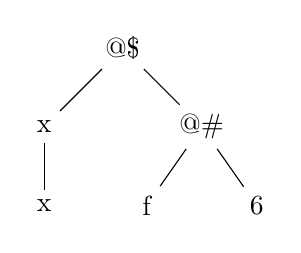
\begin{tikzpicture}
        \node (ats) at (0,   0)  {\ml{@\$}};
        \node (lam) at (-1, -1)  {\ml{\tl x}};
        \node (atr) at (1,  -1)  {\ml{@\#}};
        \node (x)   at (-1, -2)  {\ml{x}};
        \node (f)   at (0.3,-2)  {\ml{f}};
        \node (six) at (1.7,-2)  {\ml{6}};
        \draw (ats) -- (lam);
        \draw (ats) -- (atr);
        \draw (lam) -- (x);
        \draw (atr) -- (f);
        \draw (atr) -- (six);
    \end{tikzpicture}
    \vspace{-0.5\baselineskip}
}

There are two ways in which we can update the root of the redex:

\begin{numbered}
    \item We could \textit{copy the root cell of the result} on top of the root cell of the redex
    thus:

    \plainbox{
        \centering
        \raisebox{-\height}{%
            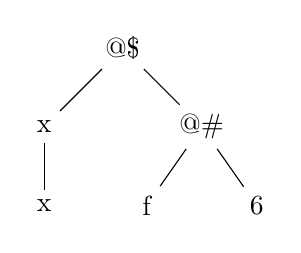
\begin{tikzpicture}
                \node (ats) at (0,   0)  {\ml{@\$}};
                \node (lam) at (-1, -1)  {\ml{\tl x}};
                \node (atr) at (1,  -1)  {\ml{@\#}};
                \node (x)   at (-1, -2)  {\ml{x}};
                \node (f)   at (0.3,-2)  {\ml{f}};
                \node (six) at (1.7,-2)  {\ml{6}};
                \draw (ats) -- (lam);
                \draw (ats) -- (atr);
                \draw (lam) -- (x);
                \draw (atr) -- (f);
                \draw (atr) -- (six);
            \end{tikzpicture}%
        }%
        \raisebox{-\height}{reduces to\hspace{1cm}}%
        \raisebox{-\height}{%
            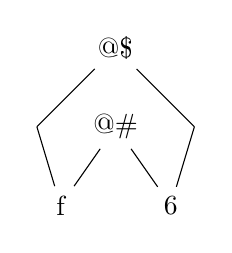
\begin{tikzpicture}
                \node (ats) at (0,    0)  {\ml{@\$}};
                \node (atr) at (0,   -1)  {\ml{@\#}};
                \node (f)   at (-0.7,-2)  {\ml{f}};
                \node (six) at (0.7, -2)  {\ml{6}};
                \node [draw=none] (phantom_l) at (-1, -1) {};
                \node [draw=none] (phantom_r) at (1,  -1) {};
                \draw (phantom_l.center) -- (ats) -- (phantom_r.center);
                \draw (phantom_l.center) -- (f);
                \draw (phantom_r.center) -- (six);
                \draw (atr) -- (f);
                \draw (atr) -- (six);
            \end{tikzpicture}
        }
    }

    Now the result (seen from the point of view of node \ml{\$}) is quite correct
    (viz.\ \ml{(f 6)}). However, now the application of \ml{f} to \ml{6} has been duplicated,
    \ml{(f 6)} \textit{may be evaluated twice} if node \ml{\#} happens to be shared. This would be
    wasted work if \ml{(f 6)} were expensive; we have lost laziness. Notice that this
    problem can only arise if the body of the lambda abstraction consists of a
    single variable. If the body is an application, then the root of the result
    will be a newly constructed application cell, and hence cannot be shared.

    \phantom{XX} Even if this were not the case, and the \ml{(f 6)} were already in normal
    form, node \ml{\$} is a duplicate of node \ml{\#}, which is a waste of storage space.

    \phantom{XX} Furthermore, this alternative might not be possible in an implementation supporting variable-sized cells, if the root cell of the argument was
    bigger than the root cell of the redex.

    \item We could take the hint from Section~12.4.1, and use an indirection node.
    We would then overwrite node \ml{\$} with an indirection to node \ml{\#}, thus:

    \plainbox{
        \centering
        \raisebox{-\height}{%
            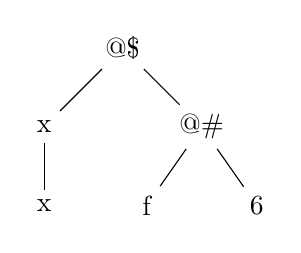
\begin{tikzpicture}
                \node (ats) at (0,   0)  {\ml{@\$}};
                \node (lam) at (-1, -1)  {\ml{\tl x}};
                \node (atr) at (1,  -1)  {\ml{@\#}};
                \node (x)   at (-1, -2)  {\ml{x}};
                \node (f)   at (0.3,-2)  {\ml{f}};
                \node (six) at (1.7,-2)  {\ml{6}};
                \draw (ats) -- (lam);
                \draw (ats) -- (atr);
                \draw (lam) -- (x);
                \draw (atr) -- (f);
                \draw (atr) -- (six);
            \end{tikzpicture}%
        }%
        \raisebox{-\height}{reduces to\hspace{1cm}}%
        \raisebox{-\height}{%
            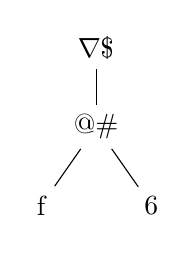
\begin{tikzpicture}
                \node (ats) at (0,   0)  {$\nabla$\ml{\$}};
                \node (atr) at (0,  -1)  {\ml{@\#}};
                \node (f)   at (-0.7,-2) {\ml{f}};
                \node (six) at (0.7,-2)  {\ml{6}};
                \draw (ats) -- (atr);
                \draw (atr) -- (f);
                \draw (atr) -- (six);
            \end{tikzpicture}%
        }
    }

    \noindent The trouble with introducing indirection nodes is that they can then
    appear at any point in the graph, so the reduction machine must contain
    tests for indirection nodes in many places.

    \phantom{XX} Furthermore there is a danger that long chains of indirection nodes
    might build up (for example, suppose \ml{(f 6)} evaluated to an indirection
    node), which would clog up the machine.
\end{numbered}

The issue of whether to copy or to use indirection nodes arises in other cases
also. For example, \ml{HEAD} selects the head of its argument (which it first
evaluates to a \ml{CONS} cell), and meets the same problem in overwriting the root
of the redex with the result. \ml{IF} is another example of such a function.
Functions like these which simply select some component of their
argument(s) are called \textit{projection functions}.

All the arithmetic and boolean functions will suffer too in an unboxed
implementation, because their result is unboxed.

In general, any function whose result is not a cell constructed during the
reduction will raise the question of how to update the root.

\subsection{Evaluating the Result before Updating}

A solution which overcomes the major problems of either method is \textit{to
    evaluate} the result \textit{before} updating the root of the redex. We can justify this
approach with the following two observations:

\begin{numbered}
    \item We are currently trying to reduce node \ml{\$} to weak head normal form. So
    the first thing we are going to do once this reduction is complete is to
    reduce the result of the reduction (\ml{(f 6)} in this case) to WHNF.

    \phantom{XX} Hence we can safely reduce node \ml{\#} to WHNF \textit{before} overwriting node
    \ml{\$} with the result.

    \item Once an expression is in WHNF its root is never again overwritten,
    because it is never again selected as the root of a redex.
\end{numbered}
Observation (i) means that if the result of the reduction of node \ml{\#} was an
indirection to a \ml{CONS} cell \ml{*}, we could overwrite node \ml{\$} with an indirection to
node \ml{*} (not node \ml{\#}).

\plainbox{
    \centering
    \raisebox{-\height}{%
        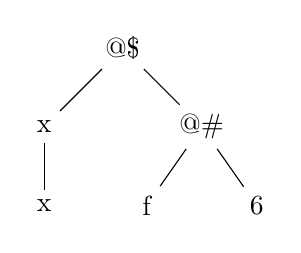
\begin{tikzpicture}
            \node (ats) at (0,   0)  {\ml{@\$}};
            \node (lam) at (-1, -1)  {\ml{\tl x}};
            \node (atr) at (1,  -1)  {\ml{@\#}};
            \node (x)   at (-1, -2)  {\ml{x}};
            \node (f)   at (0.3,-2)  {\ml{f}};
            \node (six) at (1.7,-2)  {\ml{6}};
            \draw (ats) -- (lam);
            \draw (ats) -- (atr);
            \draw (lam) -- (x);
            \draw (atr) -- (f);
            \draw (atr) -- (six);
        \end{tikzpicture}%
    }%
    \raisebox{-\height}{reduces to\hspace{1cm}}%
    \raisebox{-\height}{%
        \begin{tikzpicture}
            \node (ats)  at (-1.25,    0)  {$\nabla$ \ml{\$}};
            \node (atrn) at (-1,   -1)  {$\nabla$\ml{\#}};
            \node (star) at (1.25, -2)  {\ml{:\ *}};
            \node (p)    at (.3,   -3)  {\ml{p}};
            \node (q)    at (2, -3)  {\ml{q}};
            \node [draw=none] (phantom_l) at (-0.4, -2) {};
            \node [draw=none] (phantom_r) at (0,  0) {};
            \draw (ats) -- (phantom_r.center);
            \draw (atrn) -- (phantom_l.center);
            \draw (phantom_l.center) -- (star);
            \draw (phantom_r.center) -- (star);
            \draw (star) -- (p);
            \draw (star) -- (q);
        \end{tikzpicture}%
    }
}

\noindent Thus we would never get more than one indirection node in a chain.

Observation (ii) tells us that it is safe to copy node \ml{\#} once it is in WHNF
since it will never again be overwritten; by copying it we still waste space, but
we no longer risk duplicated reductions. For example, if the \ml{(f 6)} evaluated to
a \ml{CONS} cell, copying would give this:

\plainbox{
    \centering
    \raisebox{-\height}{%
        \begin{tikzpicture}
            \node (ats) at (0,   0)  {\ml{@}};
            \node (lam) at (-1, -1)  {\ml{\tl x}};
            \node (atr) at (1,  -1)  {\ml{@}};
            \node (x)   at (-1, -2)  {\ml{x}};
            \node (f)   at (0.3,-2)  {\ml{f}};
            \node (six) at (1.7,-2)  {\ml{6}};
            \draw (ats) -- (lam);
            \draw (ats) -- (atr);
            \draw (lam) -- (x);
            \draw (atr) -- (f);
            \draw (atr) -- (six);
        \end{tikzpicture}%
    }%
    \raisebox{-\height}{reduces to\hspace{1cm}}%
    \raisebox{-\height}{%
        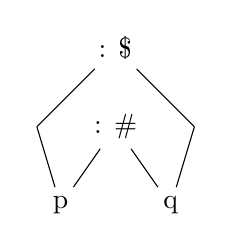
\begin{tikzpicture}
            \node (ats) at (0,    0)  {\ml{: \$}};
            \node (atr) at (0,   -1)  {\ml{: \#}};
            \node (p)   at (-0.7,-2)  {\ml{p}};
            \node (q) at (0.7, -2)  {\ml{q}};
            \node [draw=none] (phantom_l) at (-1, -1) {};
            \node [draw=none] (phantom_r) at (1,  -1) {};
            \draw (phantom_l.center) -- (ats) -- (phantom_r.center);
            \draw (phantom_l.center) -- (p);
            \draw (phantom_r.center) -- (q);
            \draw (atr) -- (p);
            \draw (atr) -- (q);
        \end{tikzpicture}
    }
}

\subsection{Summary: Indirection Nodes versus Copying}

This is a slightly tricky section, and we shall summarize our conclusions.

\begin{numbered}
    \item When the root of the result is constructed during the reduction, and is
    sufficiently small, it should be constructed directly on top of the root of
    the redex, rather than being allocated elsewhere, copied and discarded.
    \item If the root of the result was not constructed during the reduction, then we
    can overwrite the root of the redex \textit{either} with a copy of the root of
    the result, \textit{or} with an indirection to the result.
    \item The cases covered by (ii) arise for
    \begin{compactenum}[(a)]
        \item functions (both lambda abstractions and built-in functions)
        returning unboxed results,
        \item lambda abstractions whose body consists of a single variable,
        \item built-in projection functions, which include \ml{HEAD}, \ml{TAIL} and \ml{IF}.
    \end{compactenum}
    \item In the cases covered by (ii), the result should be evaluated to WHNF
    before overwriting the root of the redex. If this is done, no sharing is lost
    and the number of reductions performed is the same either way.
\end{numbered}

There are the following arguments in favor of using indirections:

\begin{numbered}
    \item There is no alternative if the result is an unboxed object.
    \item They use no fewer cells at the time the reduction takes place. However,
    indirection nodes can be `shorted out' and recovered by the garbage
    collector, thus recovering the storage they occupy, whereas the garbage
    collector cannot recover the duplicated storage allocated by the copying
    technique (see Chapter~17).
    \item There is no problem if the root of the result is bigger than the root of the
    redex.
    \item Chains of indirection nodes can be prevented.
    \item It has been suggested by Hughes [1985] that implementations of
    functional languages should incorporate \textit{memo functions}; that is,
    functions which remember what arguments they have been applied to so
    far, together with the corresponding results, and when reapplied to one
    of these arguments deliver the corresponding result directly. This idea
    works better in a system based on indirection nodes, since if we make
    copies of nodes then identical arguments may look different to the memo
    function.
\end{numbered}

There is only one argument against indirection nodes, but it is rather
persuasive:

\begin{numbered}
    \item The reduction machine has to make continual tests for the presence of
    indirection nodes, and de-reference them as they crop up. This adds a
    large number of potentially slow tests to the implementation. Hardware
    support would largely alleviate this problem.
\end{numbered}

\noindent On balance it looks as if copying has a short-term advantage of speed, but the
generality of indirection will probably win out in the end.

\section{Implementing Y}

We have said in Chapter~2 that \ml{Y} is always implemented directly, and we now
discuss how this is done. The reduction rule for \ml{Y} is
\begin{letalign}
    \ml{Y f} & \reduction{} \ml{f (Y f)}
\end{letalign}
and there are two ways of implementing this:

\plainbox{
    (i) \quad
    \raisebox{-\height}{%
        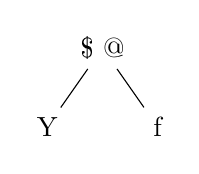
\begin{tikzpicture}
            \node (ats) at (0,  0)  {\ml{\$ @}};
            \node (Y)   at (-0.7,-1) {\ml{Y}};
            \node (f)   at (0.7,-1)  {\ml{f}};
            \draw (ats) -- (Y);
            \draw (ats) -- (f);
        \end{tikzpicture}%
    } \quad
    \raisebox{-\height}{\hspace{0.5cm}reduces to\hspace{0.5cm}}%
    \raisebox{-\height}{%
        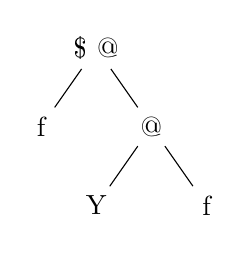
\begin{tikzpicture}
            \node (ats)  at (0,   0)  {\ml{\$ @}};
            \node (f1)   at (-0.7,-1) {\ml{f}};
            \node (atr)  at (0.7, -1) {\ml{@}};
            \node (Y)    at (0,  -2)  {\ml{Y}};
            \node (f2)   at (1.4,-2)  {\ml{f}};
            \draw (ats) -- (f1);
            \draw (ats) -- (atr);
            \draw (atr) -- (Y);
            \draw (atr) -- (f2);
        \end{tikzpicture}%
    }
    \vs

    \hspace{-20pt}\noindent\rule{\linewidth+20pt}{0.75pt}

    (ii) \quad
    \raisebox{-\height}{%
        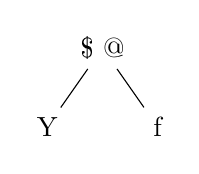
\begin{tikzpicture}
            \node (ats) at (0,  0)  {\ml{\$ @}};
            \node (Y)   at (-0.7,-1) {\ml{Y}};
            \node (f)   at (0.7,-1)  {\ml{f}};
            \draw (ats) -- (Y);
            \draw (ats) -- (f);
        \end{tikzpicture}%
    } \quad
    \raisebox{-\height}{\hspace{0.5cm}reduces to\hspace{0.5cm}}%
    \raisebox{-\height}{%
        \begin{tikzpicture}[>={Stealth[scale=1.5]}]
            \node (ats) at (0,   0)  {\ml{\$ @}};
            \node (f)   at (-0.7,  -1)  {\ml{f}};
            \node [draw=none] (phantom_a) at (.7, -1) {};
            \node [draw=none] (phantom_b) at (1.7, -1) {};
            \node [draw=none] (phantom_c) at (1.7, 0.7) {};
            \node [draw=none] (phantom_d) at (0, 0.7) {};
            \draw (phantom_a.center) -- (ats) -- (f);
            \draw (phantom_a.center) -- (phantom_b.center) -- (phantom_c.center);
            \draw (phantom_c.center) -- (phantom_d.center);
            \draw[->] (phantom_d.center) -- (ats);
        \end{tikzpicture}%
    }
}

\noindent The first is straightforward, but the second is more interesting. The right
branch of the result node \ml{\$} points back at node \ml{\$}. To see that this is a correct
implementation, consider the reduction rule for \ml{Y}. On the right-hand side of
the rule, the thing \ml{f} is applied to is \ml{(Y f)}, but the \textit{original} redex was \ml{(Y f)} and so
\ml{f} can be applied to the root of the original redex.

Another way to see this is to try taking the reduction sequence for \ml{Y} further:
\begin{letalign}
    \ml{Y f} & \reduction{} \ml{f (Y f)} \\
    & \reduction{} \ml{f (f (Y f))} \\
    & \reduction{} \ml{f (f (f (Y f)))} \\
    &$\cdots$ \\
    & \reduction{} \ml{f (f (f ($\cdots$)))}
\end{letalign}
which is just what the suggested graph represents.

This is the first time our graphs have incorporated \textit{cycles} and this is indeed
the only source of cycles in many implementations. This form of \ml{Y} is therefore
sometimes called \textit{cyclic} Y or \textit{knot-tying} Y.

Cyclic graphs give important economies in the use of storage. Using the
acyclic version of \ml{Y} means that the graph representing \ml{(Y f)} grows without
limit as each recurrent \ml{(Y f)} redex is evaluated. In contrast, using a cyclic
version of \ml{Y} means that \ml{(Y f)} is represented by a single cell. Hence cyclic
graphs give finite representations of some infinite objects (such as recursive
functions and some infinite data structures).

The principal disadvantage of a cyclic \ml{Y} is that the presence of cycles
prevents the use of simple reference-counting garbage collection (see Chapter
17).

\section*{References}

\begin{references}

    \item Hughes, R.J.M. 1985. Lazy memo functions. In \textit{Proceedings of the IFIP Conference on
        Functional Programming Languages and Computer Architecture, Nancy}, pp.
    129--46. Jouannaud (editor). LNCS 201. Springer Verlag. September.

    \item Mago, G.A. 1980. A cellular computer architecture for functional programming.
    \textit{IEEE Computer Society COMPCON}, pp. 179--87.

    \item Wadsworth, C.P. 1971. Semantics and pragmatics of the lambda calculus, Chapter 4.
    PhD thesis, Oxford.

\end{references}